\documentclass[12pt,a4paper]{report}
\usepackage[utf8]{inputenc}
\usepackage{amsmath}
\usepackage{amsfonts}
\usepackage{amssymb}
\usepackage{amsthm}
\usepackage{hyperref}

\usepackage{multicol}
\usepackage{fancyhdr}
\usepackage[inline]{enumitem}
\usepackage{tikz}
\usepackage{tikz-cd}
\usetikzlibrary{calc}
\usetikzlibrary{shapes.geometric}
\usepackage[margin=0.5in]{geometry}
\usepackage{xcolor}
\usepackage{listings} 

\usepackage{pgfplots}
\hypersetup{
    colorlinks=true,
    linkcolor=blue,
    filecolor=magenta,      
    urlcolor=cyan,
    pdftitle={Tensors},
    pdfpagemode=FullScreen,
    }

%\urlstyle{same}

\newcommand{\CLASSNAME}{Math 5301 -- Numerical Analysis}
\newcommand{\STUDENTNAME}{Paul Carmody}
\newcommand{\ASSIGNMENT}{Final Project }
\newcommand{\DUEDATE}{May 8, 2025}
\newcommand{\SEMESTER}{Spring 2025}
\newcommand{\SCHEDULE}{MW 2:00 to 3:15}
\newcommand{\ROOM}{Crawford 330}

\newcommand{\MMN}{M_{m\times n}}
\newcommand{\FF}{\mathcal{F}}

\pagestyle{fancy}
 	\fancyhf{}
\chead{ \fancyplain{}{\CLASSNAME} }
%\chead{ \fancyplain{}{\STUDENTNAME} }
\rhead{\thepage}
\newcommand{\LET}{\text{Let }}
%\newcommand{\IF}{\text{if }}
\newcommand{\AND}{\text{ and }}
\newcommand{\OR}{\text{ or }}
\newcommand{\FORSOME}{\text{ for some }}
\newcommand{\FORALL}{\text{ for all }}
\newcommand{\WHERE}{\text{ where }}
\newcommand{\WTS}{\text{ WTS }}
\newcommand{\WLOG}{\text{ WLOG }}
\newcommand{\BS}{\backslash}
\newcommand{\DEFINE}[1]{\textbf{\emph{#1}}}
\newcommand{\IF}{$(\Rightarrow)$}
\newcommand{\ONLYIF}{$(\Leftarrow)$}
\newcommand{\ITH}{\textsuperscript{th} }
\newcommand{\FST}{\textsuperscript{st} }
\newcommand{\SND}{\textsuperscript{nd} }
\newcommand{\TRD}{\textsuperscript{rd} }
\newcommand{\INV}{\textsuperscript{-1} }

\newcommand{\XXX}{\mathfrak{X}}
\newcommand{\MMM}{\mathfrak{M}}
%\newcommand{\????}{\textfrak{A}}
%\newcommand{\????}{\textgoth{A}}
%\newcommand{\????}{\textswab{A}}

\DeclareMathOperator{\DER}{Der}
\DeclareMathOperator{\SGN}{sgn}

%%%%%%%
% derivatives
%%%%%%%

\newcommand{\PART}[2]{\frac{\partial #1}{\partial #2}}
\newcommand{\SPART}[2]{\frac{\partial^2 #1}{\partial #2^2}}
\newcommand{\DERIV}[2]{\frac{d #1}{d #2}}
\newcommand{\LAPLACIAN}[1]{\frac{\partial^2 #1}{\partial x^2} + \frac{\partial^2 #1}{\partial y^2}}

%%%%%%%
% sum, product, union, intersections
%%%%%%%

\newcommand{\SUM}[2]{\underset{#1}{\overset{#2}{\sum}}}
\newcommand{\PROD}[2]{\underset{#1}{\overset{#2}{\prod}}}
\newcommand{\UNION}[2]{\underset{#1}{\overset{#2}{\bigcup}}}
\newcommand{\INTERSECT}[2]{\underset{#1}{\overset{#2}{\bigcap}}}
\newcommand{\FSUM}{\SUM{n=-\infty}{\infty}}
       

%%%%%%%
% supremum and infimum
%%%%%%%

\newcommand{\SUP}[1]{\underset{#1}\sup \,}
\newcommand{\INF}[1]{\underset{#1}\inf \,}
\newcommand{\MAX}[1]{\underset{#1}\max \,}
\newcommand{\MIN}[1]{\underset{#1}\min \,}

%%%%%%%
% infinite sums, limits
%%%%%%%

\newcommand{\SUMK}{\SUM{k=1}{\infty}}
\newcommand{\SUMN}{\SUM{n=1}{\infty}}
\newcommand{\SUMKZ}{\SUM{k=0}{\infty}}
\newcommand{\LIM}[1]{\underset{#1}\lim\,}
\newcommand{\IWOB}[1]{\LIM{#1 \to \infty}}
\newcommand{\LIMK}{\IWOB{k}}
\newcommand{\LIMN}{\IWOB{n}}
\newcommand{\LIMX}{\IWOB{x}}
\newcommand{\NIWOB}{\LIM{n \to \infty}}
\newcommand{\LIMSUPK}{\underset{k\to\infty}\limsup \,}
\newcommand{\LIMSUPN}{\underset{n\to\infty}\limsup \,}
\newcommand{\LIMINFK}{\underset{k\to\infty}\liminf \,}
\newcommand{\LIMINFN}{\underset{n\to\infty}\liminf \,}
\newcommand{\ROOTRULE}[1]{\LIMSUPK \BARS{#1}^{1/k}}

\newcommand{\CUPK}{\bigcup_{k=1}^{\infty}}
\newcommand{\CAPK}{\bigcap_{k=1}^{\infty}}
\newcommand{\CUPN}{\bigcup_{n=1}^{\infty}}
\newcommand{\CAPN}{\bigcap_{n=1}^{\infty}}

%%%%%%%
% number systems (real, rational, etc.)
%%%%%%%

\newcommand{\REALS}{\mathbb{R}}
\newcommand{\RATIONALS}{\mathbb{Q}}
\newcommand{\IRRATIONALS}{\REALS \backslash \RATIONALS}
\newcommand{\INTEGERS}{\mathbb{Z}}
\newcommand{\NUMBERS}{\mathbb{N}}
\newcommand{\COMPLEX}{\mathbb{C}}
\newcommand{\DISC}{\mathbb{D}}
\newcommand{\HPLANE}{\mathbb{H}}

\newcommand{\R}{\mathbb{R}}
\newcommand{\Q}{\mathbb{Q}}
\newcommand{\Z}{\mathbb{Z}}
\newcommand{\N}{\mathbb{N}}
\newcommand{\C}{\mathbb{C}}
\newcommand{\T}{\mathbb{T}}
\newcommand{\COUNTABLE}{\aleph_0}
\newcommand{\UNCOUNTABLE}{\aleph_1}


%%%%%%%
% Arithmetic/Algebraic operators
%%%%%%%


\DeclareMathOperator{\MOD}{mod}
%\newcommand{\MOD}[1]{\mod #1}
\newcommand{\BAR}[1]{\overline{#1}}
\newcommand{\LCM}{\text{ lcm}}
\newcommand{\ZMOD}[1]{\Z/#1\Z}
\DeclareMathOperator{\VAR}{Var}
%%%%%%%
% complex operators
%%%%%%%

\DeclareMathOperator{\RR}{Re}
%\newcommand{\RE}{\text{Re}}
\DeclareMathOperator{\IM}{Im}
%\newcommand{\IM}{\text{Im}}
\newcommand{\CONJ}[1]{\overline{#1}}
\DeclareMathOperator{\LOG}{Log}
%\newcommand{\LOG}{\text{ Log }}
\newcommand{\RES}[2]{\underset{#1}{\text{res}} #2}

%%%%%%%
% Group operators
%%%%%%%

\newcommand{\AUT}{\text{Aut}\,}
\newcommand{\KER}{\text{ker}\,}
\newcommand{\END}{\text{End}}
\newcommand{\HOM}{\text{Hom}}
\newcommand{\CYCLE}[1]{(\begin{array}{cccccccccc}
		#1
	\end{array})}
\newcommand{\SUBGROUP}{\underset{\text{group}}\subseteq}	
%\newcommand{\SUBGROUP}{\subseteq_g}
\newcommand{\SUBRING}{\underset{\text{ring}}\subseteq}
\newcommand{\SUBMOD}{\underset{\text{mod}}\subseteq}
\newcommand{\SUBFIELD}{\underset{\text{field}}\subseteq}
\newcommand{\ISO}{\underset{\text{iso}}\longrightarrow}
\newcommand{\HOMO}{\underset{\text{homo}}\longrightarrow}

%%%%%%%
% grouping (parenthesis, absolute value, square, multi-level brackets).
%%%%%%%

\newcommand{\PAREN}[1]{\left (\, #1 \,\right )}
\newcommand{\BRACKET}[1]{\left \{\, #1 \,\right \}}
\newcommand{\SQBRACKET}[1]{\left [\, #1 \,\right ]}
\newcommand{\ABRACKET}[1]{\left \langle\, #1 \,\right \rangle}
\newcommand{\BARS}[1]{\left |\, #1 \,\right |}
\newcommand{\DBARS}[1]{\left \| \, #1 \,\right \|}
\newcommand{\LBRACKET}[1]{\left \{ #1 \right .} 
\newcommand{\RBRACKET}[1]{\left . #1 \right \]}
\newcommand{\RBAR}[1]{\left . #1 \, \right |}
\newcommand{\LBAR}[1]{\left | \, #1 \right .}
\newcommand{\BLBRACKET}[2]{\BRACKET{\RBAR{#1}#2}}
\newcommand{\GEN}[1]{\ABRACKET{#1}}
\newcommand{\BINDEF}[2]{\LBRACKET{\begin{array}{ll}
     #1\\
     #2
\end{array}}}

%%%%%%%
% Fourier Analysis
%%%%%%%

\newcommand{\ONEOTWOPI}{\frac{1}{2\pi}}
\newcommand{\FHAT}{\hat{f}(n)}
\newcommand{\FINT}{\int_{-\pi}^\pi}
\newcommand{\FINTWO}{\int_{0}^{2\pi}}
\newcommand{\FSUMN}[1]{\SUM{n=-#1}{#1}}
%\newcommand{\FSUM}{\SUMN{\infty}}
\newcommand{\EIN}[1]{e^{in#1}}
\newcommand{\NEIN}[1]{e^{-in#1}}
\newcommand{\INTALL}{\int_{-\infty}^{\infty}}
\newcommand{\FTINT}[1]{\INTALL #1 e^{2\pi inx\xi} dx}
\newcommand{\GAUSS}{e^{-\pi x^2}}

%%%%%%%
% formatting 
%%%%%%%

\newcommand{\LEFTBOLD}[1]{\noindent\textbf{#1}}
\newcommand{\SEQ}[1]{\{#1\,\}}
\newcommand{\WIP}{\footnote{work in progress}}
\newcommand{\QED}{\hfill\square}
\newcommand{\ts}{\textsuperscript}
\newcommand{\HLINE}{\noindent\rule{7in}{1pt}\\}

%%%%%%%
% Mathematical note taking (definitions, theorems, etc.)
%%%%%%%

\newcommand{\REM}{\noindent\textbf{\\Remark: }}
\newcommand{\DEF}{\noindent\textbf{\\Definition: }}
\newcommand{\THE}{\noindent\textbf{\\Theorem: }}
\newcommand{\COR}{\noindent\textbf{\\Corollary: }}
\newcommand{\LEM}{\noindent\textbf{\\Lemma: }}
\newcommand{\PROP}{\noindent\textbf{\\Proposition: }}
\newcommand{\PROOF}{\noindent\textbf{\\Proof: }}
\newcommand{\EXP}{\noindent\textbf{\\Example: }}
\newcommand{\TRICKS}{\noindent\textbf{\\Tricks: }}


%%%%%%%
% text highlighting
%%%%%%%

\newcommand{\B}[1]{\textbf{#1}}
\newcommand{\CAL}[1]{\mathcal{#1}}
\newcommand{\UL}[1]{\underline{#1}}

%%%%%%
% Linear Algebra
%%%%%%

\newcommand{\COLVECTOR}[1]{\PAREN{\begin{array}{c}
#1
\end{array} }}
\newcommand{\TWOXTWO}[4]{\PAREN{ \begin{array}{c c} #1&#2 \\ #3 & #4 \end{array} }}
\newcommand{\DTWOXTWO}[4]{\BARS{ \begin{array}{c c} #1&#2 \\ #3 & #4 \end{array} }}
\newcommand{\THREEXTHREE}[9]{\PAREN{ \begin{array}{c c c} #1&#2&#3 \\ #4 & #5 & #6 \\ #7 & #8 & #9 \end{array} }}
\newcommand{\DTHREEXTHREE}[9]{\BARS{ \begin{array}{c c c} #1&#2&#3 \\ #4 & #5 & #6 \\ #7 & #8 & #9 \end{array} }}
\newcommand{\NXN}{\PAREN{ \begin{array}{c c c c} 
			a_{11} & a_{12} & \cdots & a_{1n} \\
			a_{21} & a_{22} & \cdots & a_{2n} \\
			\vdots & \vdots & \ddots & a_{1n} \\
			a_{n1} & a_{n2} & \cdots & a_{nn} \\
		\end{array} }}
\newcommand{\SLR}{SL_2(\R)}
\newcommand{\GLR}{GL_2(\R)}
\DeclareMathOperator{\TR}{tr}
\DeclareMathOperator{\BIL}{Bil}
\DeclareMathOperator{\SPAN}{span}

%%%%%%%
%  White space
%%%%%%%

\newcommand{\BOXIT}[1]{\noindent\fbox{\parbox{\textwidth}{#1}}}


\newtheorem{theorem}{Theorem}[section]
\newtheorem{corollary}{Corollary}[theorem]
\newtheorem{lemma}[theorem]{Lemma}

\theoremstyle{definition}
\newtheorem{definition}[theorem]{Definition}
\newtheorem{prop}[theorem]{Proposition}

\theoremstyle{remark}
\newtheorem{remark}[theorem]{Remark}
\newtheorem{example}[theorem]{Example}
%\newtheorem*{proof}[theorem]{Proof}



\newcommand{\RED}[1]{\textcolor{red}{#1}}
\newcommand{\BLUE}[1]{\textcolor{blue}{#1}}
\definecolor{mygreen}{RGB}{28,172,0} % color values Red, Green, Blue
\definecolor{mylilas}{RGB}{170,55,241}

\begin{document}
\lstset{language=Matlab,%
    %basicstyle=\color{red},
    breaklines=true,%
    morekeywords={matlab2tikz},
    keywordstyle=\color{blue},%
    morekeywords=[2]{1}, keywordstyle=[2]{\color{black}},
    identifierstyle=\color{black},%
    stringstyle=\color{mylilas},
    commentstyle=\color{mygreen},%
    showstringspaces=false,%without this there will be a symbol in the places where there is a space
    numbers=left,%
    numberstyle={\tiny \color{black}},% size of the numbers
    numbersep=9pt, % this defines how far the numbers are from the text
    emph=[1]{for,end,break},emphstyle=[1]\color{red}, %some words to emphasise
    %emph=[2]{word1,word2}, emphstyle=[2]{style},    
}

\begin{center}
	\Large{\CLASSNAME -- \SEMESTER} \\
	\large{ w/Professor Du}
\end{center}
\begin{center}
	\STUDENTNAME \\
	\ASSIGNMENT -- \DUEDATE\\
\end{center} 
\HLINE

\begin{center}
	\textbf{\Large{Interpretation of Polling Data from \\Micro-controller input sensors.}}\\
\end{center} 

Micro-controllers are often the first line of detection and active response to the environment.  These are triggered through sensors that deliver a stream of data that must be interpreted before the properly coded response can be triggered.  The data stream can fluctuate on a moment by moment basis but display overall aggregated behavior that is useful for an application.  That is, the input data must be interpreted in order to give reliability of input data strenth that can then be used to determine responses.  The data is interpreted through the integral of the polling data over time using the Simpson’s Rule.\\

\noindent Assumptions and parameters:
\begin{enumerate}
	\item The data may be quite different between each measurement but changes smoothly.
	\item The change in data (i.e., first derivative) also changes smoothly.
	\item Make available \textit{parameters of reliability}.  These would give some indication as to the effect of accuracy and processor efficiency.
	\item Attempts should be made to optimize where the greatest changes occur.
	\item Reduce as small as possible, the 'software footprint', i.e., the amount of space used for processing and data.\footnote{Micro-controllers have very limited space for code and data for interpretation which must be shared with response subroutines.}\\
\end{enumerate}

\newcommand{\SECTION}[1]{\noindent\textbf{\Large{#1}}}
\newcommand{\SUBSECTION}[1]{\noindent\textbf{#1}}\SECTION{Simpson's 1/3 Rule\\}

Because of the first two assumptions mentioned above, we can approximate each node of data with quadratic interpolation.  That is, given two-endpoints we can take the midpoint and interpolate a quadratic curve, $P(x)$, with the following approximation:\footnote{https://en.wikipedia.org/wiki/Simpsons\_rule\#Composite\_Simpson's\_1/3\_rule}\\
\begin{minipage}{0.5\textwidth}
\begin{align*}
	\int_a^b f(x)dx &\approx P_m\\
	P_m &= \frac{b-a}{6}\SQBRACKET{f(a)+4f(m)+f(b)}
\end{align*}where $m=\frac{a+b}{2}$.  The graphs shows the quadratic interpolation $P(x)$ in red.
\end{minipage}
\begin{minipage}{0.5\textwidth}
\begin{center}

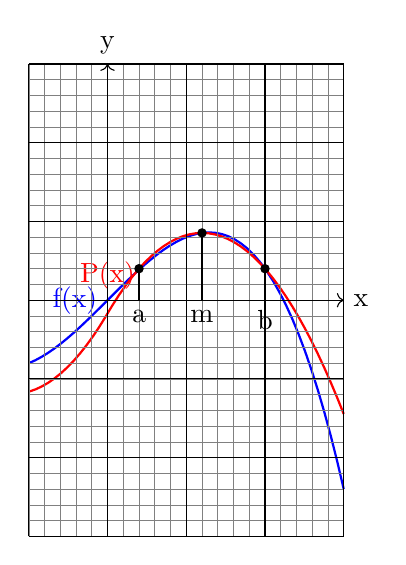
\begin{tikzpicture}
  \draw[domain=-1:3,samples=50,color=blue,thick] node[left] {f(x)} plot (\x, -\x^3/5 + \x);
 %P(x) = −0.710x^2 +1.704x−0.168
  \draw[domain=-1:3,samples=50,color=red,thick] node[above] {P(x)} plot (\x, -0.710*\x^2+1.704*\x-0.168);
  \draw[very thin,gray,step=.2] (-1,-3) grid (3,3);
  \draw[step=1] (-1,-3) grid (3,3);
  \draw[->] (-1,0) -- (3,0) node[right] {x};
  \draw[->] (0,-3) -- (0,3) node[above] {y};
  \draw[thick,black] (0.4,0.4) -- (0.4,0) node[below] {a};
  \draw[thick,black] (1.2,0.8544) -- (1.2,0) node[below] {m};
  \draw[thick,black] (2,0.4) -- (2,0) node[below] {b};
  \foreach \x/\y in { 0.4/0.4, 1.2/0.8544, 2/0.4}
    \fill (\x,\y) circle (0.6mm);
\end{tikzpicture}
\end{center}
\end{minipage}

\SUBSECTION{Error Analysis of Simpson's Rule.\\}

The error for approximating via Simpon's Rule for $n=2$ is 
\begin{align*}
	-\frac{1}{90}h^5f^{(4)}(\xi) = -\frac{(b-a)^5}{2880}f^{(4)}(\xi), \text{ for some } \xi \in [a,b], h=\frac{b-a}{2}
\end{align*}``Since the error term is proportional to the fourth derivative of $f$ at $\xi$ this shows that Simpon's Rule provides exact solutions for polynomial $f$ of degree three or less, since the fourth derivative of such a polyomial is zero at all points."\footnote{https://en.wikipedia.org/wiki/Simpsons\_rule\#Composite\_Simpson's\_1/3\_rule}  Sensors used for micro-controllers usually are concerned with motion detection, infrared intensity, temperature, humidity, etc. this is a reasonable assumption that acceleration (in the case of motion as an example) would be a constant or change linearly and for a short interval ($<0.001$ seconds).\\

\SUBSECTION{Verification of Simpson's Rule\\}

Because Simpson's rule gives accurate approximations to the third derivative, we need only verify quadratic interpolations.  We can see that each of the terms of a quadratic are true with each of these terms
\begin{itemize}
	\item The Constant Term:
	\begin{align*}
		f(x) &= 1\\
		\int_a^b dx &= (b-a)\\
		P_m &=  \frac{b-a}{6} \PAREN{1+4+1} = b-a
	\end{align*}
	\item The Linear Term:
	\begin{align*}
		f(x) &= x \\
		\int_a^b ax dx &= x^2|_a^b \\
		&= \frac{b^2-a^2}{2} \\
		P_m &= \frac{b-a}{6} \PAREN{b+\frac{a+b}{2}+a} = \frac{b-a}{6} (3b+3a) \\
		&= \frac{b^2-a^2}{2}
	\end{align*}
	\item The Quadratic Term:
	\begin{align*}
		f(x) &= x^2\\
		\int_a^b x^2 dx &= \frac{1}{3}x^3 |_a^b\\
		&= \frac{b^3-a^3}{3}\\
		P_m &= \frac{b-a}{6}\PAREN{a^2+4\PAREN{\frac{a+b}{2}}^2 + b^2}\\
		&= \frac{b-a}{6}\PAREN{a^2+\PAREN{a^2+2ab+b^2} + b^2}\\
		&= \frac{b-a}{3}\PAREN{a^2+2ab+b^2} \\
		&= \frac{b^3-a^3}{3}
	\end{align*}
\end{itemize}

This evidence of Simpson's Rule on a single interval.  These can be further refined by greater subdivisions and a resulting collection of quadratic interpolated elements (see the section on "Testing and Perfomance", below).  This would lead to matrix of qudratic solutions that could increase complexity.   However, we will see that a recursive approach will provide for greater efficiencies and more information and fulfill the requirements for the "Assumptions and Parameters" mentioned above. \\

\SECTION{A Recursive Solution.\\}

  Input data may appear more eratic than smooth as in this graph (and perhaps not as regular):

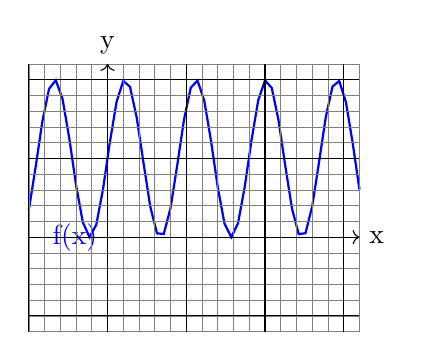
\begin{tikzpicture}
  \draw[domain=-1:3.2,samples=50,color=blue,thick] node[left] {f(x)} plot (\x, {sin(deg(\x*7))+1});
  \draw[very thin,gray,step=.2] (-1,-1.2) grid (3.2,2.2);
  \draw[step=1] (-1,-1.2) grid (3.2,2.2);
  \draw[->] (-1,0) -- (3.2,0) node[right] {x};
  \draw[->] (0,-0.2) -- (0,2.2) node[above] {y};
\end{tikzpicture}\\

By requirement \#4 from above, "Attempts should be made to optimize where the greatest changes occur", we can improve our efficiency by focusing our algorithm on sections that appear to have more activity.  For this reason, instead of coding an interative approach with a finer poling data, we'll use a recursive approach dependent on the tolerance level of the overall estimated element.  That is, if the estimate $m(b-a)$ is within tolerance range of $P(m)$ then we may stop.  Otherwise, the interval is split into two intervals $[a,m]$ and $[m,b]$ and recursively called again.  In this way, intervals with more eratic behavior will be further subdivided while those with smooth behavior will be quickly estimated.\\

\SUBSECTION{Efficiency and Accuracy of Recursion.\\}

\textbf{Depth and Iterations.}  In a typical interative algorithm, cost and efficiency depend entirely on how often complicated calculations are made.  This is true for a recursive solution as well, but an additional value, namely depth, offers us some measure of complexity or volatility that is not as easily available in a standard iterative solution.  \\

\textbf{Definition: } Define the \textbf{depth, d} as the number of recursive calls before the tolerance level has been met.\\

The greater the depth the more recursions were required to make for an acceptable estimate.  Clearly, if the data is smooth there will be fewer estimations needed.  As the data is more eratic more recursions are needed and the depth increases.  By returning the depth of the calculation we get a measure of the "noise" or "level of volatility" of the input data.\\

\textbf{Definition: } Define the \textbf{iterations, I} as the number of tests throughout the calculation.\\

Each recursive step constitutes one iteration, but might not require another recursive call (i.e., adding one to the depth).  It is easy to see that a greater depth with fewer iterations indicates an isolation of volatile data (e.g., a data spike) and smaller depth in relations to the iterations indicates a smoother and more consistent data set.  So, in addition to the estimate of the integral of $f$ over $[a,b]$ we gain information on smoothness, consistency and volaltiliy.  This is additional information at no cost to efficeincy that might be helpful contributing towards response to the environment.\\

\textbf{Efficiency. } Micro-controllers have very small capacity for memory (e.g., Arduino has only 32KB capacity\footnote{https://docs.arduino.cc/hardware/uno-rev3/}).  Recursive routines can be very small leaving room for data.  Further, their natural usage of stack memory recycles memory without having to manage garbage collection.  Isolating the recursive call by the tolerance reduces the number of interations based entirely on the complexity of the data returning smooth intervals more quickly and executing more cycles on more volatile data where it is needed.\\

\textbf{Lag Time. } Micro-processors poll their sensors at 10K per second while the processor speed is 16 MHz, thus the lag time between measurement and evaluation depends greatly on the sample size.  With the measurements of depth and iterations, the application can dynamically respond to sample size in order to gain a more timely response. \\

\textbf{Caveat.  } It is possible that in a given sub-interval the midpoint could provide a value within tolerance of the expected value despite the fact that the interval might contain volatile data.  Thus, passing the tolerance test, no deeper recursive calls are made.  The depth, $d$, can serve as a confidence in calculation if other indicators do not support a lower volatility of data.  Granularity of recursive calls, that is, instead of subdividing into two interval subdivide into 3 or 4 can be done on a per application basis, further reducing the potential for this mishap.  Or, simply, compare the current results with the previous results for consistency.

\SECTION{\\The Algorithm.\\}

For the purposes of this paper, the code listed here is in MatLab.  The implementation code will be for that of the native language for the micro-controller (typically a version of C).  \\

\lstinputlisting{simpson.m}

\SECTION{\\Testing and Performance.\\}

Performance testing must include the following criteria:
\begin{itemize}
	\item Test 1: \textbf{Verify that integration is accurate.}
	
	Equation: $y=1$\\
	Interval:  $[0, 4]$.\\
	Expectations:  Expected results: 4 and short depth and iterations
	
	\item Test 2: Simple curves that show quick response.
	
	Equation: $y=x^2$\\
	Interval: $[0, 4]$.\\
	Expectation:  Expected results: 21.333 and short depth and iterations
	
	\item Test 3: Slightly more complex curves indicate more intricate responses (i.e., greater depth).
	
	Equation: $y= |\sin(x)|$\\
	Interval: $[0, \pi/2]$.\\
	Expectation:  result: 1, Increased depth and iterations.
	
	\item Test 4: Very volatile data.  Great variations in value indicating greater depth and interations.
	
	Equation: $y= \sin(11x)+1$\\
	Interval: $[0, \pi/2]$.\\
	Expectation: Result: 1.57, increased depth and iteration values.
	
	\item Test 5: Partitioned data values with no relation to each other.  This should indicate a mixture of depth and iterative values from previous tests.
	
	Equation:
	\begin{align*}
		y = \BINDEF{x & 0< x< \pi/4}{\sin(11x)+1 & \pi/4 < i < \pi/2}
	\end{align*}\\
	Interval: $[0,\pi/2]$\\
	Expection: result: 1.142, a mixture of depth and iteration values.
\end{itemize}

\SUBSECTION{Graphs of the Test Data\\}
\begin{minipage}{0.3\textwidth}
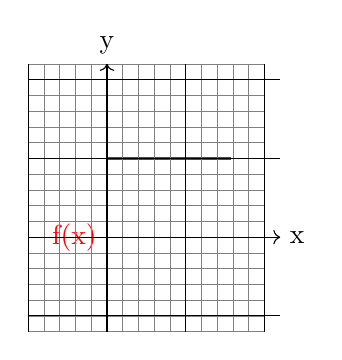
\begin{tikzpicture}
  \draw[domain=0:1.58,samples=50,color=red,thick] node[left] {f(x)} plot (\x, {1});
  \draw[very thin,gray,step=.2] (-1,-1.2) grid (2.0,2.2);
  \draw[step=1] (-1,-1.2) grid (2.2,2.2);
  \draw[->] (-1,0) -- (2.2,0) node[right] {x};
  \draw[->] (0,-0.2) -- (0,2.2) node[above] {y};
\end{tikzpicture}\\Test 1: $y=1$
\end{minipage}
\begin{minipage}{0.3\textwidth}
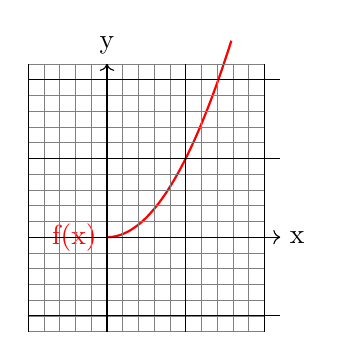
\begin{tikzpicture}
  \draw[domain=0:1.58,samples=50,color=red,thick] node[left] {f(x)} plot (\x, {\x^2});
  \draw[very thin,gray,step=.2] (-1,-1.2) grid (2.0,2.2);
  \draw[step=1] (-1,-1.2) grid (2.2,2.2);
  \draw[->] (-1,0) -- (2.2,0) node[right] {x};
  \draw[->] (0,-0.2) -- (0,2.2) node[above] {y};
\end{tikzpicture}\\Test 2: $y=x^t$
\end{minipage}
\begin{minipage}{0.3\textwidth}
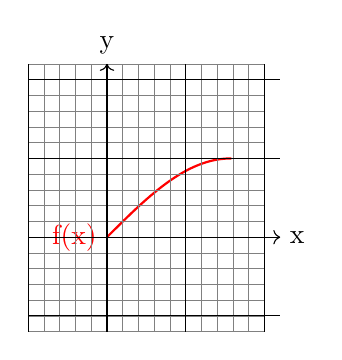
\begin{tikzpicture}
  \draw[domain=0:1.58,samples=50,color=red,thick] node[left] {f(x)} plot (\x, {abs(sin(deg(\x)))});
  \draw[very thin,gray,step=.2] (-1,-1.2) grid (2.0,2.2);
  \draw[step=1] (-1,-1.2) grid (2.2,2.2);
  \draw[->] (-1,0) -- (2.2,0) node[right] {x};
  \draw[->] (0,-0.2) -- (0,2.2) node[above] {y};
\end{tikzpicture}\\Test 3: $y=|\sin(x)|$
\end{minipage}\\
\begin{minipage}{0.3\textwidth}
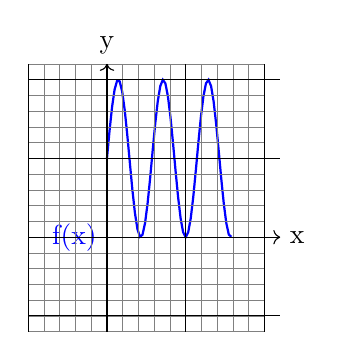
\begin{tikzpicture}
  \draw[domain=0:1.58,samples=50,color=blue,thick] node[left] {f(x)} plot (\x, {sin(deg(\x*11))+1});
  \draw[very thin,gray,step=.2] (-1,-1.2) grid (2.0,2.2);
  \draw[step=1] (-1,-1.2) grid (2.2,2.2);
  \draw[->] (-1,0) -- (2.2,0) node[right] {x};
  \draw[->] (0,-0.2) -- (0,2.2) node[above] {y};
\end{tikzpicture}\\Test 4: $\sin(11x)+1$
\end{minipage}
\begin{minipage}{0.3\textwidth}
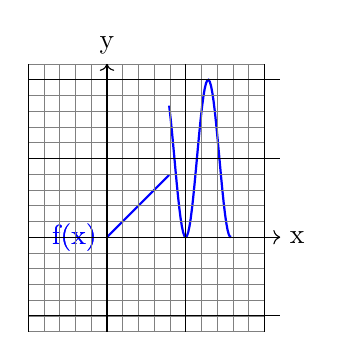
\begin{tikzpicture}
  \draw[domain=0:0.79,samples=50,color=blue,thick] node[left] {f(x)} plot (\x, {\x});
  \draw[domain=0.79:1.58,samples=50,color=blue,thick] node[left] {f(x)} plot (\x, {sin(deg(\x*11))+1});
  \draw[very thin,gray,step=.2] (-1,-1.2) grid (2.0,2.2);
  \draw[step=1] (-1,-1.2) grid (2.2,2.2);
  \draw[->] (-1,0) -- (2.2,0) node[right] {x};
  \draw[->] (0,-0.2) -- (0,2.2) node[above] {y};
\end{tikzpicture}\\Test 5: partitioned
\end{minipage}\\

The actual data can be more iratic and unpredictable than these samples.  These indicate the variety of potential data input and how testing reveals the response to volatility.\\

\begin{tabular}{|l|c|c|c|c|c|}
	\hline
	 	& Analytic &	 Estimated & Depth & Iteration & Accuracy \\
	 \hline
	 Test 1 & 4 & 3.996 & 1 & 2 & $99.9\%$\\
	 \hline
	 Test 2 & 21.33  & 21.566 & 9 & 161 & $98.4\%$\\
	 \hline
	 Test 3 & 1  & 1 & 5 & 30 & $100\%$\\
	 \hline
	 Test 4 & 1.57 & 1.668 & 8 & 119 & $93.8\%$\\
	 \hline
	 Test 5 & 1.142  & 1.036 & 8 & 83 & $91\%$ \\
	 \hline
\end{tabular}\\

The data supports the goal of the algorithm to spend more time on volatile areas of data and less time on smooth curves. This releases resources and processing power for the micro-controller to perform other tasks. \\

\SUBSECTION{Recursion vs Iteration.\\}

Iteration would require the complete computation of all $n$ data points regardless of the quality of the data.  This algorithm describes such a situation.

\lstinputlisting{iterate.m}

These five lines of code have a smaller processor footprint than the 35 lines of code of the recursive algorithm (after removing comments and blank lines).  And, the iterations for each calculation is always of order $o(n)$.  We can see from the table above, though, that with 1000 data points the number of iterations of the worst case is only $16\%$ of that typical iterative case.  The recursion being binary in nature, this algorithm is of order $o(\log(n))$ having much greater response time without significant loss of accuracy while providing addtional helpful information.\\


\SUBSECTION{Tolerance and Accuracy.\\}

It is worth noting that the tolerance is closely associated with the value of $h$, the incremental value between each successive node.  That is, if $h  \approx 10^{-3}$ then the accuracy is in this range for each subinterval. Taking Test 4, as an example, we can start to see that the number of wave zeros in the interval, $N$, is limited as we cannot measure any more finely. In this case, 
\begin{align*}
	\sin(Nx) &= 0 \to x = \frac{\pi}{N}, \frac{2\pi}{N}, \frac{3\pi}{N}, \dots \\
	h_{\min} &= \frac{\pi}{N} < 0.001 \to N \approx 30
\end{align*}That is, if the sensor is fluctuating wildly over 300 times a second the algorithm isn't likely to provide an accurate measure.  It is clear that volatile changes in the environment reduce the effectiveness of the algorithm.


\end{document}
